\section{Methodology}
To understand the flow behaviour of various undertray geometry, fluid dynamics analysis is required. The rapid development of computational power has allowed more accurate and reliable results in computational analysis such as computational fluid dynamics (CFD)\cite{Andersson2011ComputationalEngineers}. The usage of CFD allows engineers to simplify the processes and achieve an accurate result in shorter time which allows engineers to do more iterations. 

\begin{figure}[!htb]
    \centering
    \makebox[\textwidth]{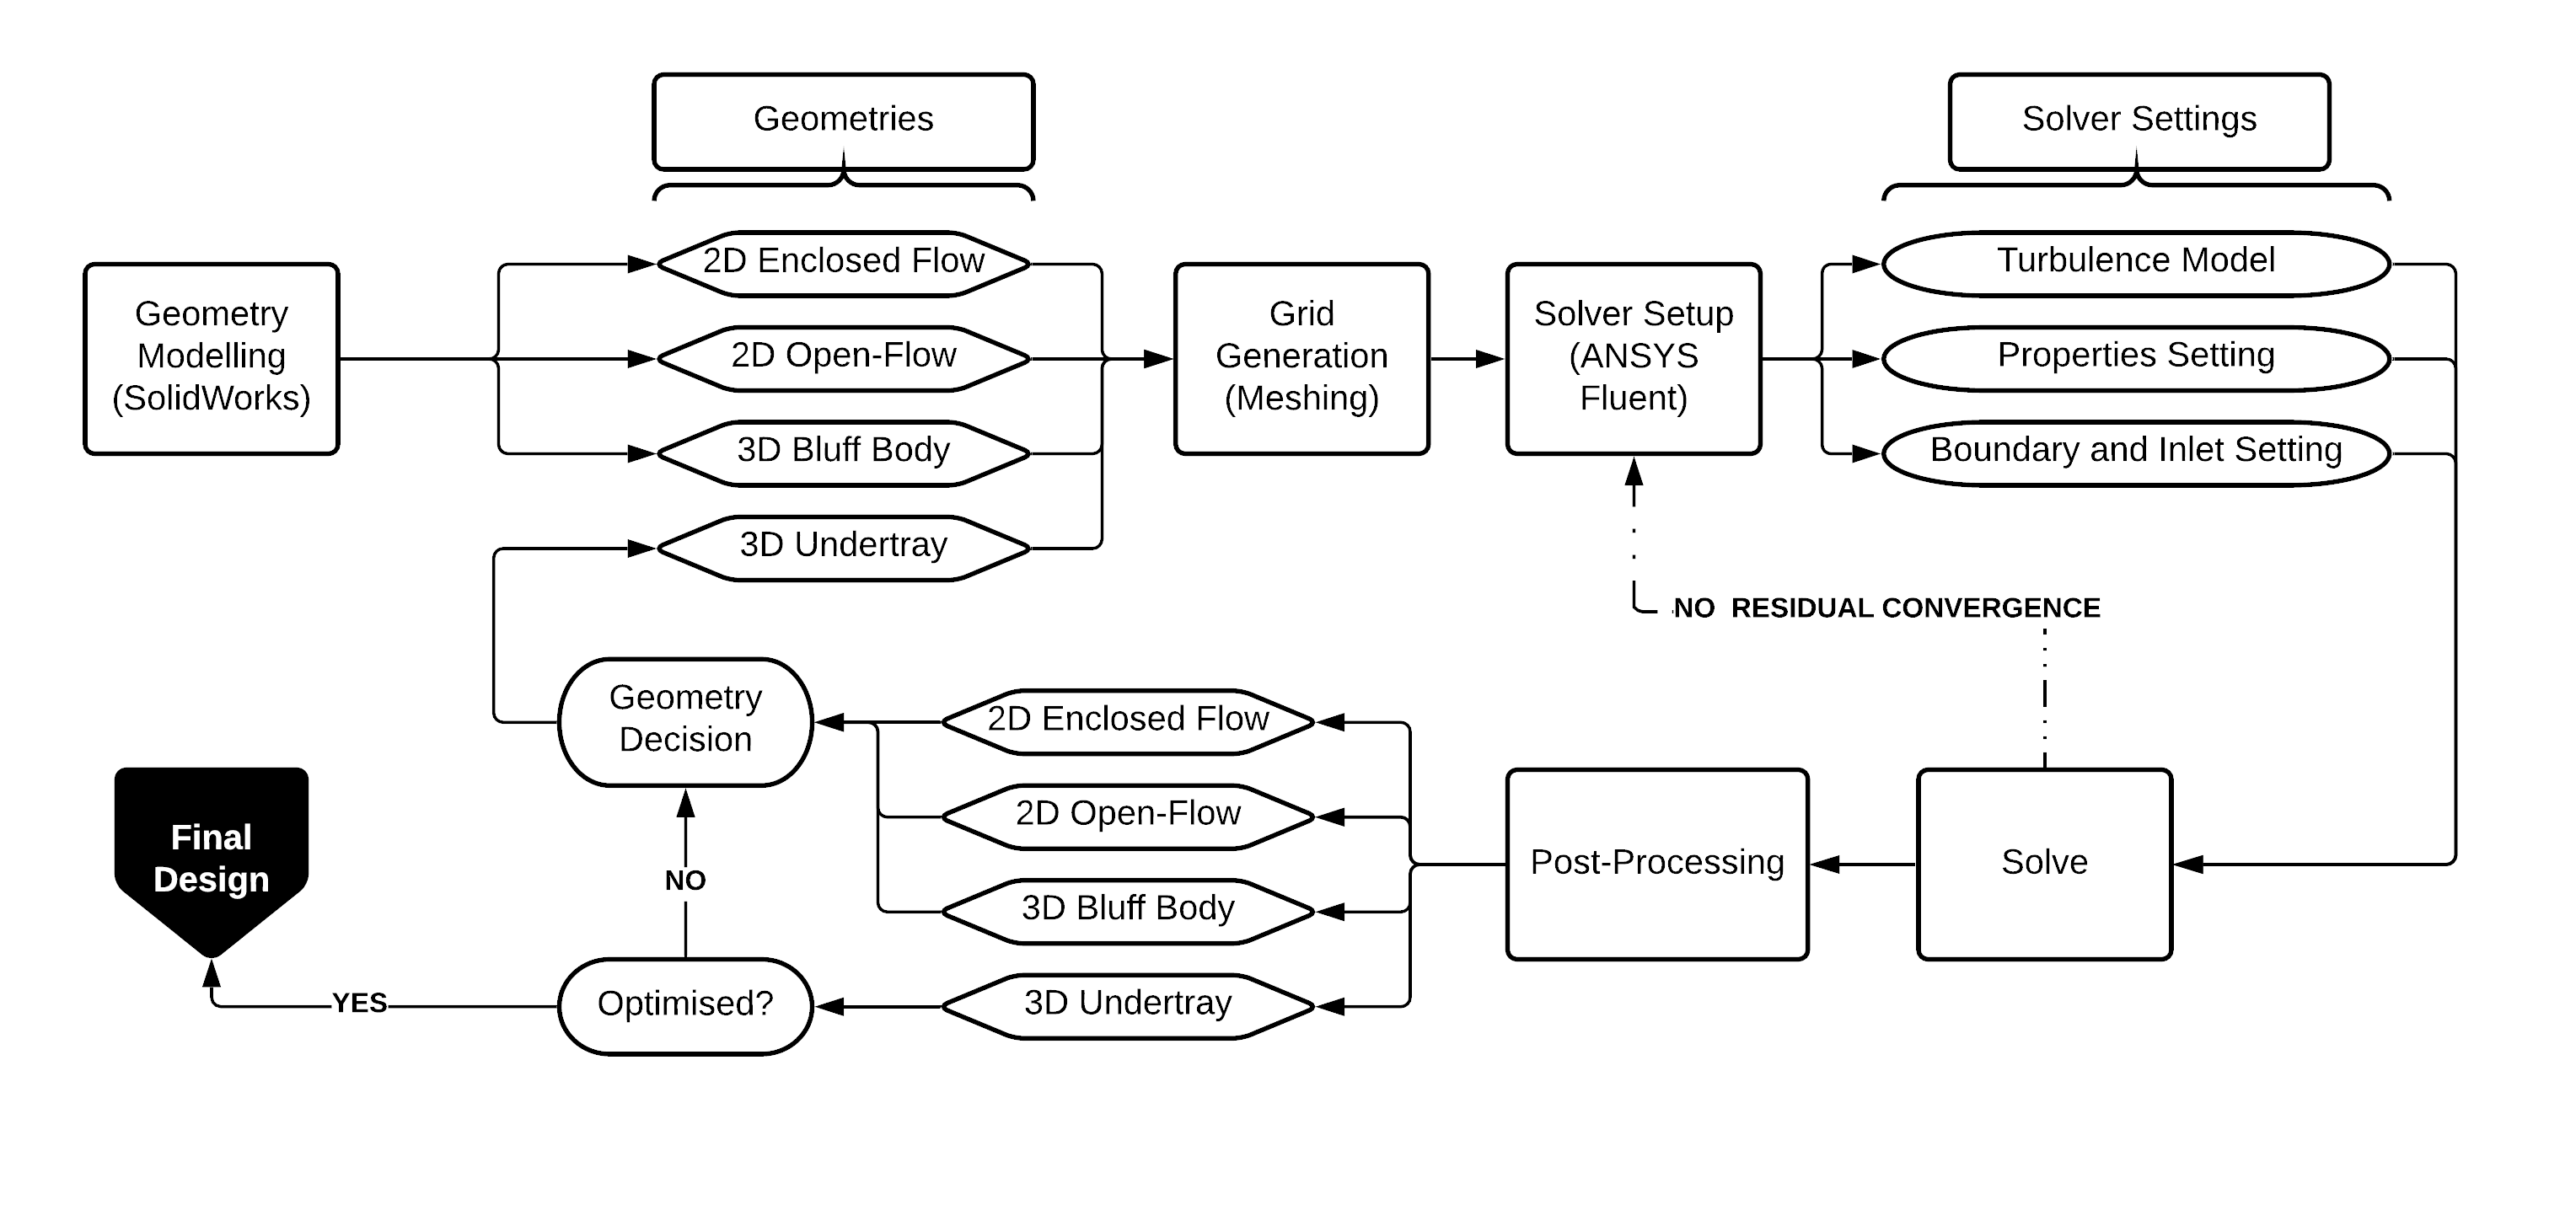
\includegraphics[scale=0.15]{Figures/project_methodology_chart.png}}
    \caption{Project Methodology Flow Chart}
    \label{fig:project methodology}
\end{figure}

\noindent The methodology consists of 3 phase which are 2D enclosed \& open-flow, 3D bluff body, 3D undertray. The first phase is the 2D analysis which analyse the undertray variables on a Venturi-tube like geometry and open-flow analysis analyse a simple bluff body with similar undertray variables. 3D bluff body will take the 2D geometry and extrude it as an 3D geometry which then analysed with the same undertray variables. Lastly is the 3D undertray where the optimised results from previous analysis will be used to determine the geometry of the final undertray design. To achieve realistic results, simplified traced body from the QFR 2021 car will be attached to the undertray. The process flow can be illustrated on figure \ref{fig:project methodology}. The work on this paper will be fully based on CFD which utilise ANSYS Fluent as a default working platform.

\subsection{Pre-Processing \& Solver Setup}

\subsubsection{Grid Generation (Meshing)}
The surface or body which have been defined from SolidWorks becomes the basis for the meshing. Meshing app which integrated in ANSYS workbench provide a user-friendly, simple, and fast meshing generator. Due to the constrain of computational power and time, unstructured triangular (2D) and tetrahedral (3D) mesh were widely used with quadrilateral (2D) and triangular prism (3D) near the wall as an inflation layer to capture the growth of boundary layer and reduce numerical diffusion \cite{Lanfrit2005BestFLUENT}.

\noindent Looking back to the goal of the 2D and 3D bluff body simulation is to obtain and analyse the trend in geometry changes of an undertray, therefore, a non-detailed yet decent mesh could be generated. Local refinement around the body that affected by the fluid flow is recommended \cite{Lanfrit2005BestFLUENT} to achieve a reasonable results and flow representation especially around the undertray, moreover this technique allows larger mesh on the far field section less likely be affected or affecting the result. Other aspect of reasonable meshing is to be aware of the mesh properties such as skewness and growth ratio. For automotive application, it is recommended to have skewness less then 0.45 and maximum growth rate less than 20\% \cite{Lanfrit2005BestFLUENT}. 

\noindent One crucial facet of an undertray flow is generation of boundary layer and how it interacts with the moving floor, the accuracy of this aspect is depend on the quality of layer grid growth near the wall or wall function. To generate a good inflation layer, it is important to make sure the y+ value (first layer height grid) does not exceed the inner boundary layer region which can be done using the equation:

\begin{equation}
    y^+ = \frac{\rho U_\tau \partial y}{\mu}, where \quad U_\tau = \sqrt{\frac{\tau_w}{\rho}} = U \sqrt{\frac{1}{2}C_f}
\end{equation}

\noindent Figure \ref{fig:inflation layer} shows the illustration of y+ value on a wall function. The turbulence model on the solver also has to be a consideration in defining the y+ value, some turbulence modelling require a very low n y+ and some are able to tolerate high y+ value. Detail regarding y+ value in various turbulent model will be discussed on the next section. 

\begin{figure}[!ht]
    \centering
    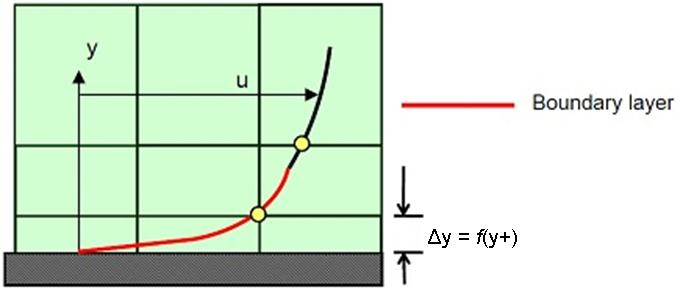
\includegraphics[height=4cm]{Figures/inflation_layer.jpg}
    \caption{Representation of y+ on a near wall function \cite{Anonymous2013Inflate4Blog}}
    \label{fig:inflation layer}
\end{figure}


\subsection{Numerical Method}
Turbulence model is a crucial aspect in approximating the unsteady turbulent fluctuation \cite{Cummings2015AppliedAerodynamics}. The quality of the turbulence modelling significantly impact the fidelity of the simulations \cite{Lanfrit2005BestFLUENT}. Due to the time constraint, variable amount, and computational power, a steady state method was used entirely in this paper. Two-equation Reynolds-Averaged Navier-Stokes (RANS) approach was also used to solve time averaged flow \cite{Cummings2015AppliedAerodynamics}. With a reasonable quality of mesh, practical lift and drag trend can be achieved which then can be studied. Realizable K-$\epsilon$ and K-$\omega$ Shear Stress Transport (SST) were used in this paper to solve the downforce and drag of the undertray and bluff body.  

\subsubsection{Realizable K-$\epsilon$  Models}
k-$\epsilon$  turbulence model is a  two-equation transport model which specifically solve the turbulence kinetic energy (k) and dissipation rate ($\epsilon$) \cite{Andersson2011Turbulent-flowModelling}\cite{Mansour1989Near-wallModeling}\cite{Ansys2006ModelingFlows}. The standard model is robust and widely-used in broad application of engineering turbulence modelling, however the nature of  k-$\epsilon$ family is not able to calculate some of the $\epsilon$ terms which can be anticipated using wall function. Moreover, k-$\epsilon$ does not perform well for flow with strong separation and large adverse pressure gradient, which the major feature of an undertray's diffuser \cite{Ansys2006ModelingFlows}.  Therefore realisable k-$\epsilon$ is broadly used in this analysis. The term 'realisable' itself allows some of mathematical satisfaction in computing the Reynolds stresses which improving its consistency of the turbulent flow. This specific transport model is crucial to capture important flow features of an undertray such as flow rotation, significant adverse pressure gradient, and vortex formation.

\subsubsection{k-$\omega$ Shear Stress Transport (SST) Models}
SST model is a 2 equation-model that combine both k-$\epsilon$ and k-$\omega$ \cite{Andersson2011Turbulent-flowModelling}\cite{Ansys2006ModelingFlows}.  k-$\epsilon$ is used in the free-stream and k-$\omega$ is used near the boundary wall means this model took the strength of both model allowing accurate prediction in all region. This model perform well on the region with adverse pressure gradient and  flow separation, moreover SST is know to have better performance compared to k-$\epsilon$ and does not required any wall function\cite{Andersson2011Turbulent-flowModelling}. However, a fine mesh ($y^+  < 5$) is required on the wall which increase the computational cost and time, as well it could over predict turbulent flow in a large strain area \cite{Andersson2011Turbulent-flowModelling}\cite{Ansys2006ModelingFlows}. 



\subsection{Boundary Conditions}
\begin{table}[!htb]
    \centering
    \caption{Boundary Conditions for 2D and 3D ANSYS Fluent setup}
    \label{tab:Boundary Conditions}
    \vspace{-0.5cm}
\begin{center}
\begin{tabular}{||p{4cm}|p{4cm}|p{7cm}||}
 \hline
 \centering
 Named Region & Boundary Condition & Property Details\\
 \hline \hline
 \multicolumn{3}{||c||}{General Properties} \\
 \hline
 
 Inlet & Inlet velocity & Velocity = 16.667 m/s (or 40 km/h)\\
 \hline
 Outlet & Outlet Pressure  & Gauge Pressure = 0 Pa  \\
 \hline
 Undertray (2D Enclosed)/Bluff Body & Stationary Wall & No-slip condition\\
 \hline
 Moving Floor & Moving Wall & Velocity = 16.667 m/s (or 40 km/h) in the flow direction\\
 \hline
 Enclosure &   Fluid (Air)  & Pressure = 101325 Pa
Temperature = 288.15 K
Density = 1.225 kg/m3
ISA Sea Level Condition\\
 
 \hline
 \multicolumn{3}{||c||}{3D Analyses} \\
 \hline
 
 Symmetry Body & Symmetry  & -\\
 \hline
 Symmetry Top & Symmetry  & -\\
 \hline
 Symmetry Side & Symmetry & -\\
 \hline
 
\end{tabular}
\end{center}
\end{table}

\noindent Table \ref{tab:Boundary Conditions} shows Boundary conditions for 2D and 3D analyses in ANSYS Fluent solver. The main goal is to simulate the flow behaviour at bottom region of the car, therefore, a moving floor was employed in all simulation with the same magnitude and direction of the flow. The usage of moving ground (or belt in wind tunnel) is a physically correct and best option to capture a ground effect such in an undertray \cite{Zhang2006GroundCars}\cite{Burgin1986WINDEFFECT}. Simulation environment was set and assumed to International Standard Atmospheric (ISA) condition at sea level. 
\vspace{1cm}
\noindent In 3 dimensional simulation, side, far-side, and top surface of the flow-field were set to symmetry where fluxes and normal gradients of all variables are assumed zero \cite{ANSYS2009SymmetryConditions} as recommended by Lanfrit \cite{Lanfrit2005BestFLUENT}. This setup along with the moving floor was surmised to provide the best results in simulating the race car or body in an actual racing track.





